\documentclass[12pt,a4paper]{report}
\usepackage[utf8]{inputenc}
\usepackage{amsmath}
\usepackage{amsfonts}
\usepackage{amssymb}
\usepackage{graphicx}
\usepackage{svg}
\usepackage{float}
\usepackage[utf8]{inputenc}
\usepackage[left=2cm,right=2cm,top=2cm,bottom=2cm]{geometry}
\renewcommand{\thesection}{\arabic{section}}
\author{Braydan Newman - n11272031}
\title{Computer Lab Portfolio}

\begin{document}
\maketitle
\tableofcontents

\newpage

\section{Week 2 - Introduction to data visualisation in MATLAB Part 1}

\subsection{Task 1}
Question: A TIFF file with the two-panel Mauna Loa CO2 graph
\\
Answer: Tiff image is in the appropriotely label week in the code folder.

\subsection{Task 2}
Question: A vector graphics file of your GBRMPA plot (e.g., EPS, SVG, PDF, etc).
\\
Answer: I did this as a SVG and couldnt find a way to show an svg through LaTeX. The file is in the appropriotely label week in the code folder.

\subsection{Task 3}

Question:A JPG file of the stack of squares in 3D, with twice as many squares in the stack
\\
Answer:
\begin{figure}[H]
\centering
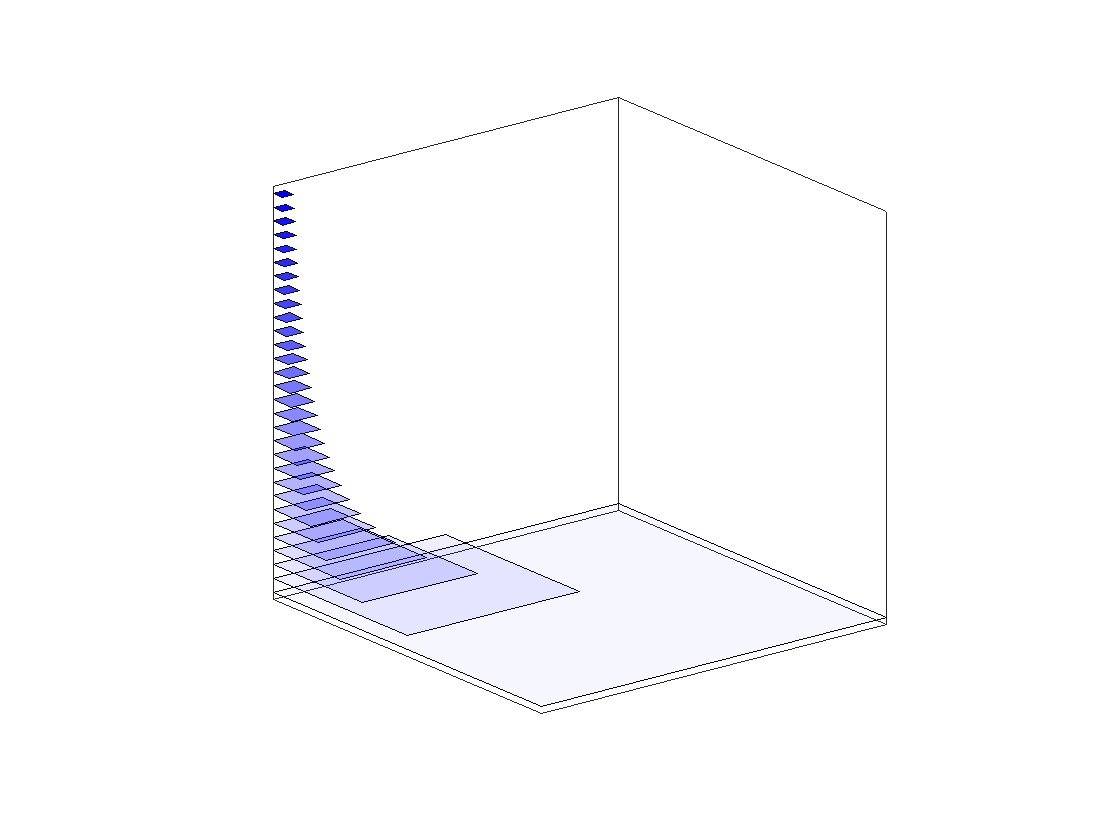
\includegraphics[width=\textwidth]{../Code/Week 2/stackSquares.jpg}
\end{figure}

\section{Week 3 - Introduction to data visualisation in MATLAB Part 2}

\subsection{Task 1}
Question: Image files (e.g., TIFF, EPS, JPEG) showing (1) a scatter plot of methamphetamine laboratory locations
superimposed on the contiguous US counties, and (2) a colour-coded map showing the relative density of
methamphetamine labs in each contiguous US state. Ensure you include axes labels, title, appropriate
fontsize, etc.
\\
Answer:

\begin{figure}[H]
\centering
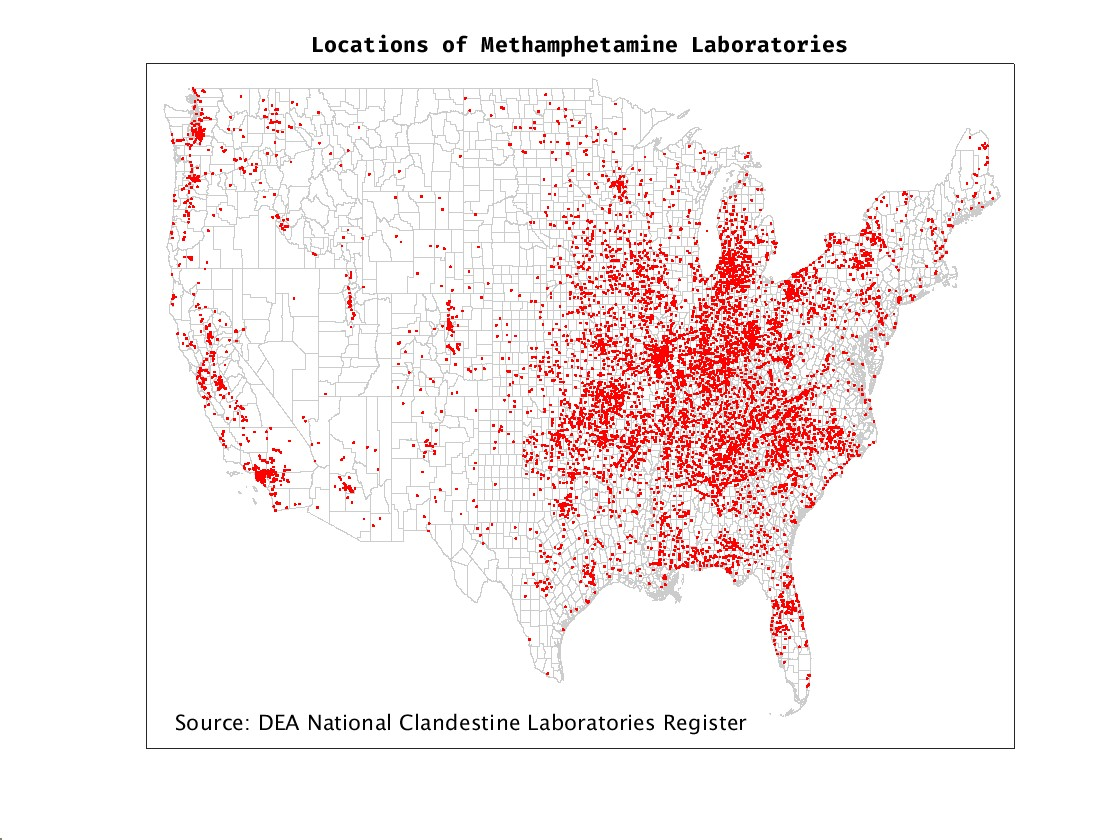
\includegraphics[width=\textwidth]{../Code/week 3/ScatterPlotMethLabs.jpg} 
\end{figure}

\begin{figure}[H]
\centering
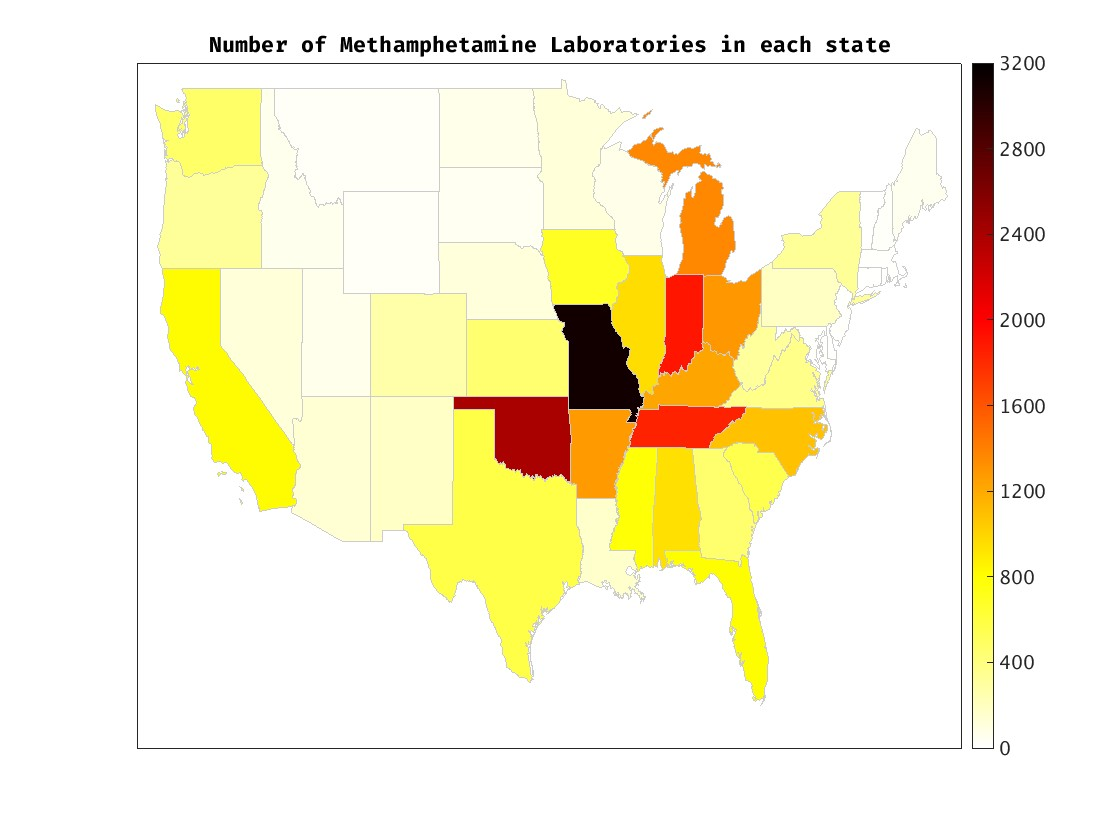
\includegraphics[width=\textwidth]{../Code/week 3/relitiveDensities.jpg}
\end{figure}
 

\subsection{Task 2}
Question: An image file showing the timeseries of the logistic mapping Nt, and also the bifurcation diagram for
values of r between 2.6 and 3.8.
\\
Answer:

\begin{figure}[H]
\centering
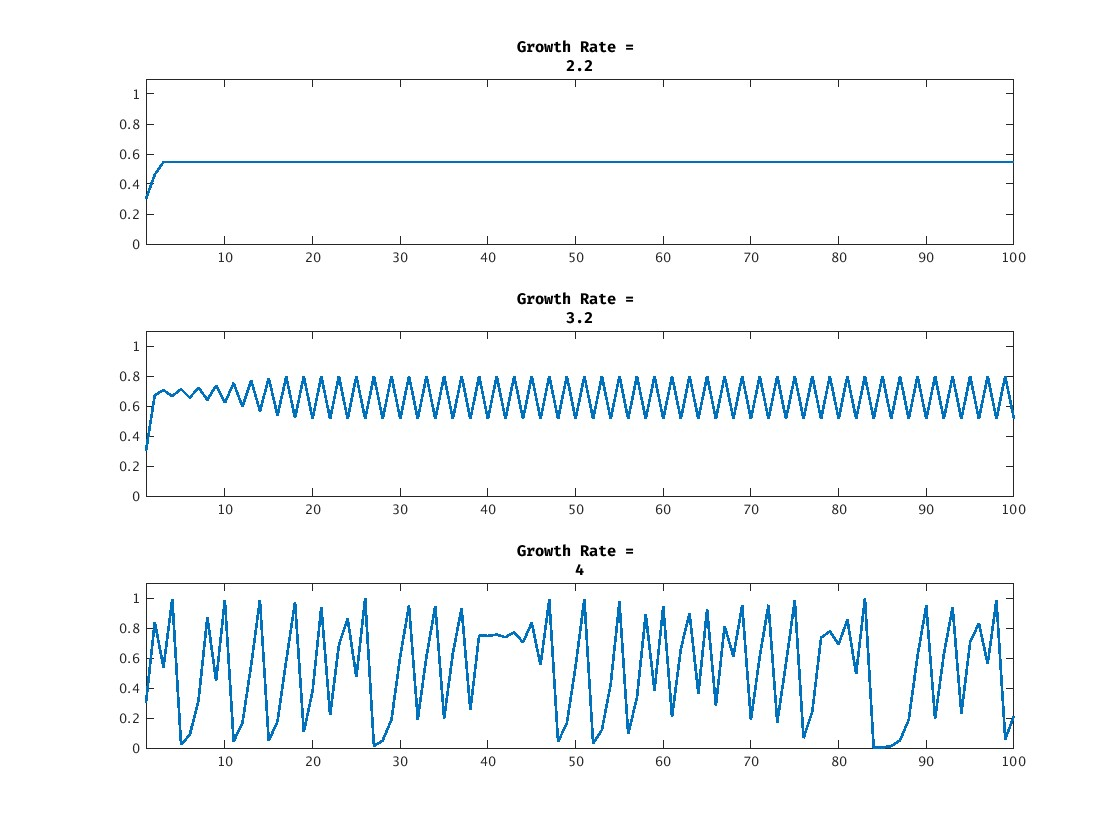
\includegraphics[width=\textwidth]{../Code/week 3/logisticMapping.jpg} 
\end{figure}

\begin{figure}[H]
\centering
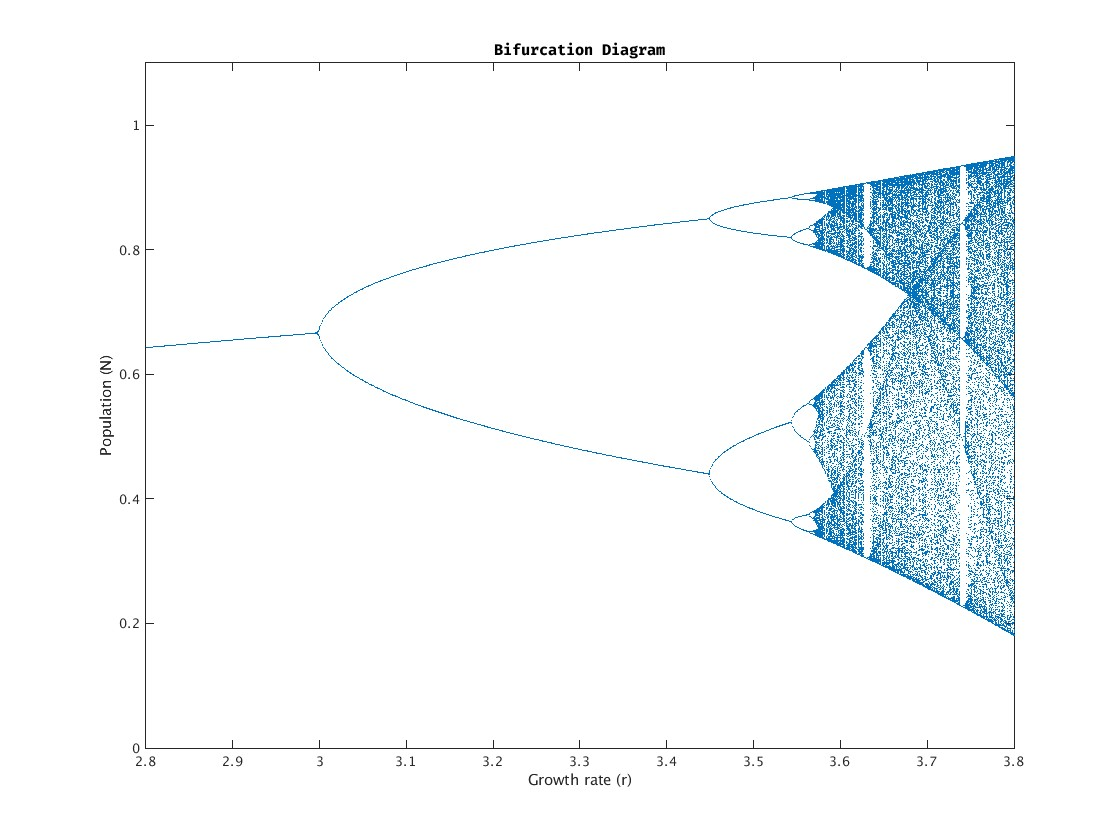
\includegraphics[width=\textwidth]{../Code/week 3/BifurcationDiagram.jpg}  
\end{figure}




\subsection{Task 3}
Question: An image of the entire Mandelbrot set, and two other images, focused on different areas.
\\
Answer:


\begin{figure}[H]
\centering
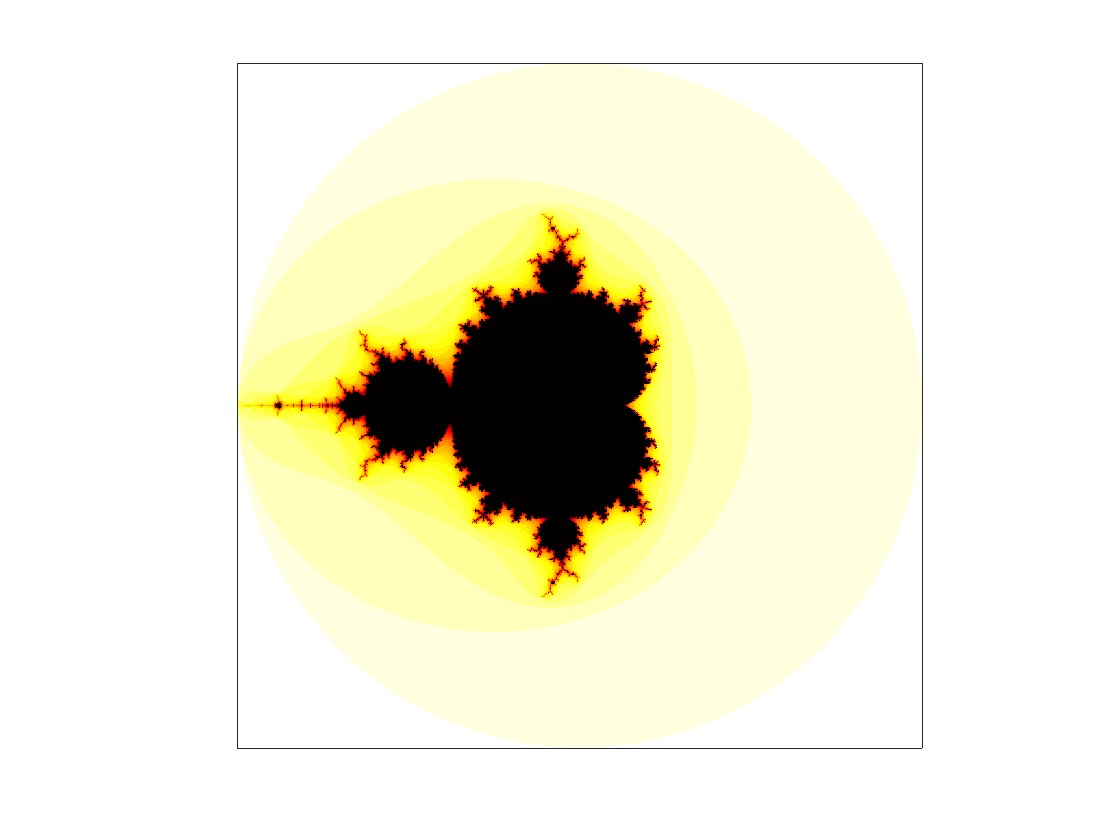
\includegraphics[width=\textwidth]{../Code/week 3/fullMadelbrot.jpg} 
\end{figure}

\begin{figure}[H]
\centering
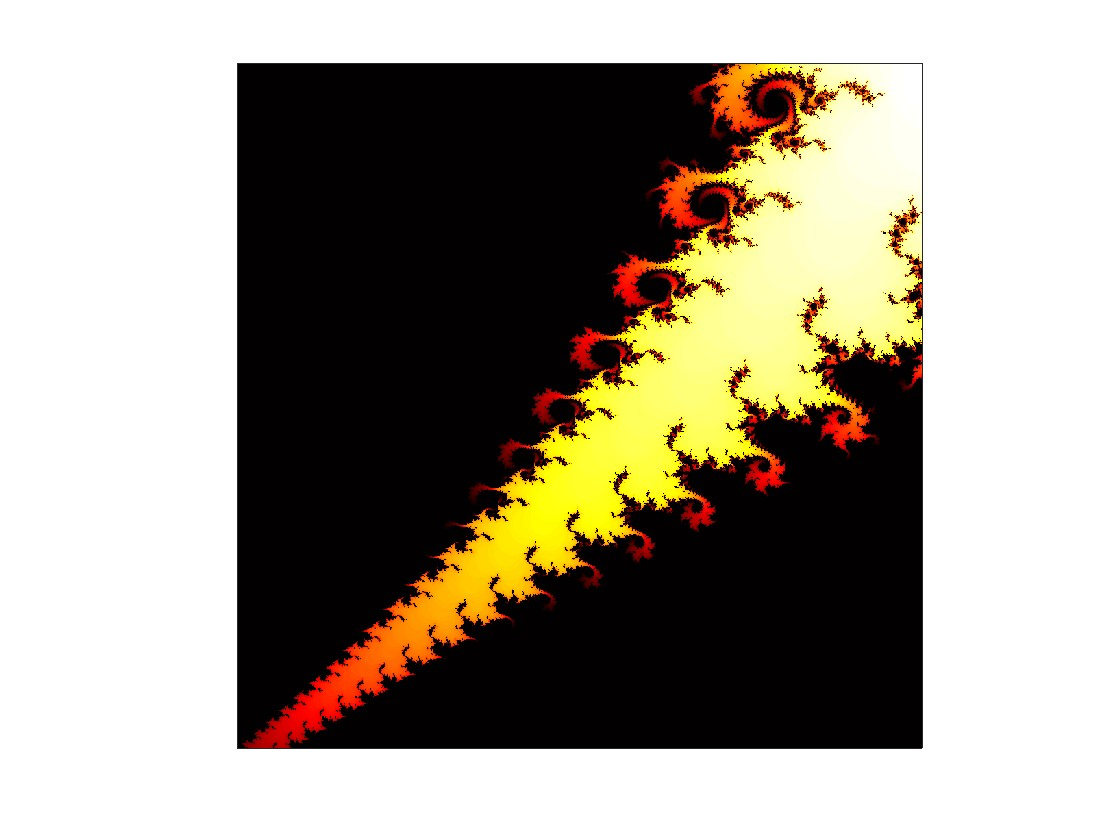
\includegraphics[width=\textwidth]{../Code/week 3/mandelbrot1.jpg} 
\end{figure}

\begin{figure}[H]
\centering
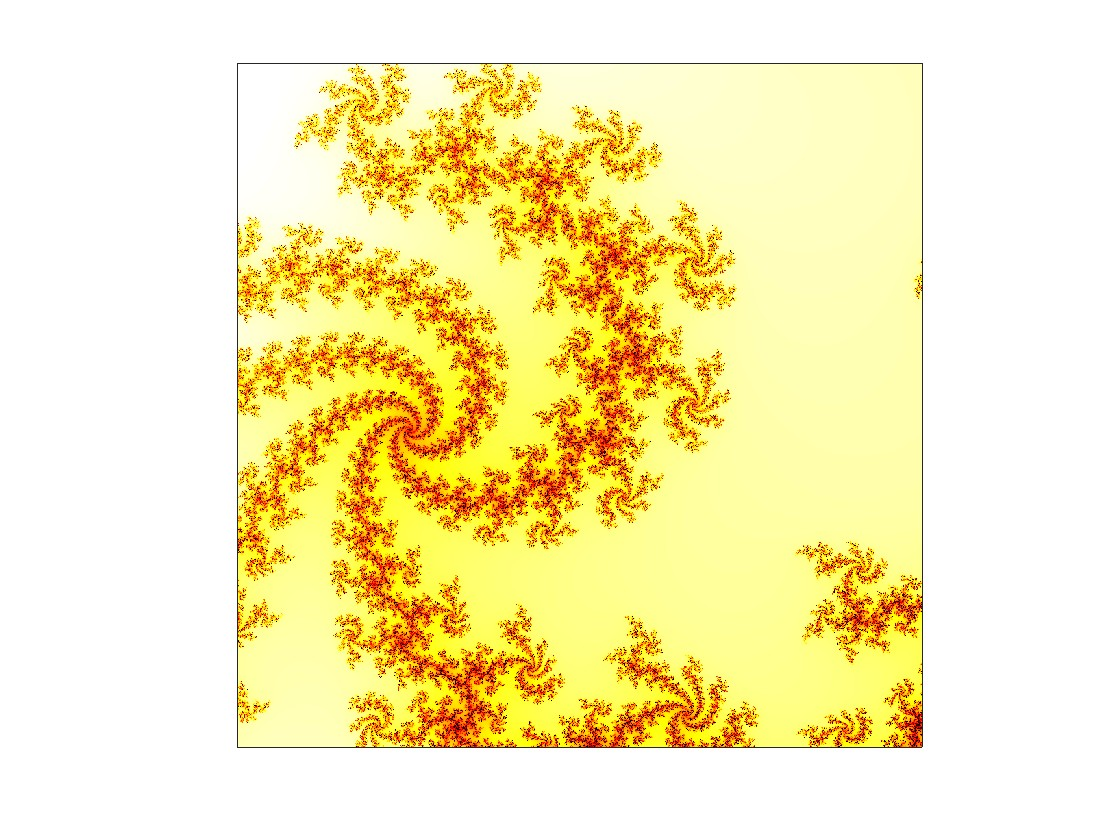
\includegraphics[width=\textwidth]{../Code/week 3/mendelbrot2.jpg} 
\end{figure}

\section{Week 5 - Animation in Matlab}
\subsection{Task 1}
Question: Produce the London population animation including all time-periods in the dataset. The resulting
animation, as an MPEG-4 file, should be included in the portfolio.
\\
Answer: I was unable to use MPEG-4 as MATLAB on Linux it is unsupported and not available, I have added it as an AVI file, which should still be accessible in most software. The file is in the appropriotely label week in the code folder.

\subsection{Task 2}
Question: Produce the pendulum animation. The resulting animation, as a GIF file, should be included in the
portfolio.
\\
Answer: I couldnt find a way to show an GIF through LaTeX. The file is in the appropriotely label week in the code folder.


\section{Week 6/8 - Volume visualisation algorithms}

\subsection{Tasks 1-4 (R Code)}
Uncomplete, was unabel to get this working.

\subsection{Tasks 1 (MATLAB Code)}
Question: A coloured isosurface of the stag beetle with an appropriately chosen ISOVALUE and viewing angle that
produce a clear volume visualisation.
\\
Answer:

\begin{figure}[H]
\centering
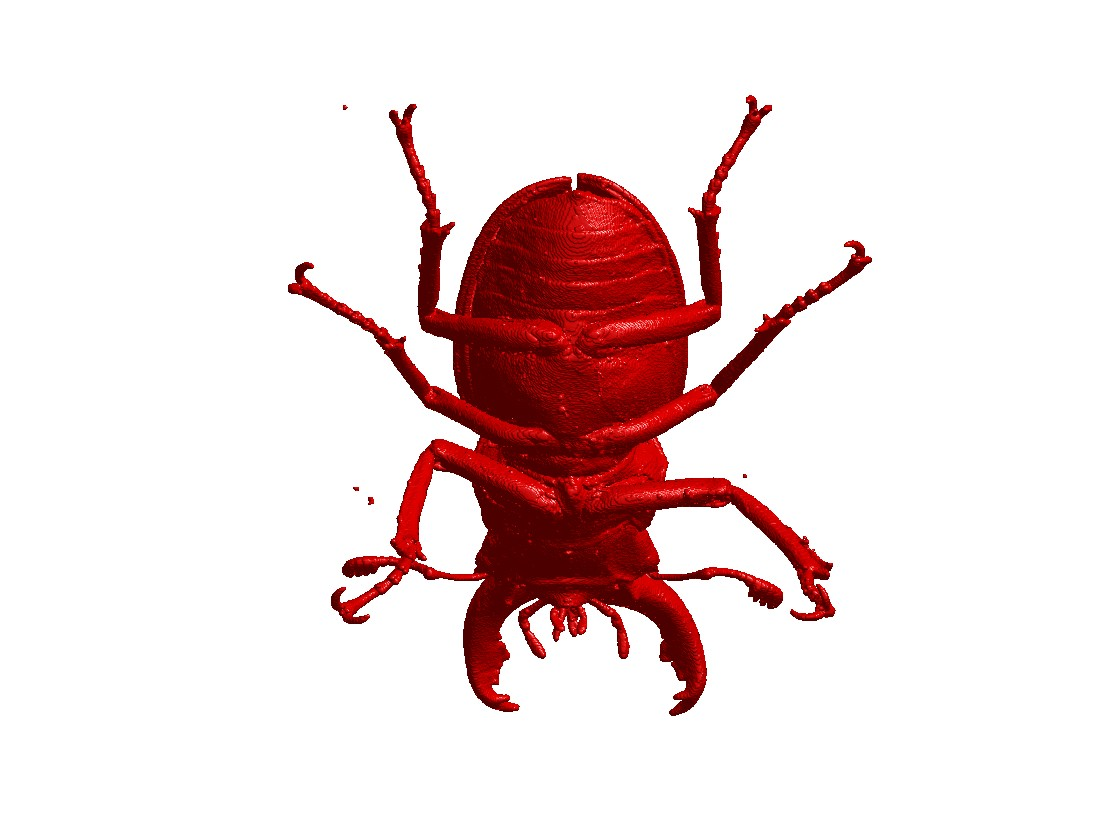
\includegraphics[width=\textwidth]{../Code/week 6/beetle.jpg} 
\end{figure}


\section{Week 9 - Visualising uncertainty}
\subsection{Task 1 (MATLAB Code)}
Question: Animation of uncertainty surrounding larval cloud through time. Does not need to be a convex hull.
\\
Answer: I couldnt find a way to show an GIF through LaTeX. The file is in the appropriotely label week in the code folder.

\subsection{Task 1 (R Code)}
Uncomplete, was unabel to get this working.

\section{Week 10 - Vector visualisation methods}
\subsection{Task 1}
Question: Direct vector field visualisation using a quiver plot (as described in Task 1).
\\
Answer: 

\begin{figure}[H]
\centering
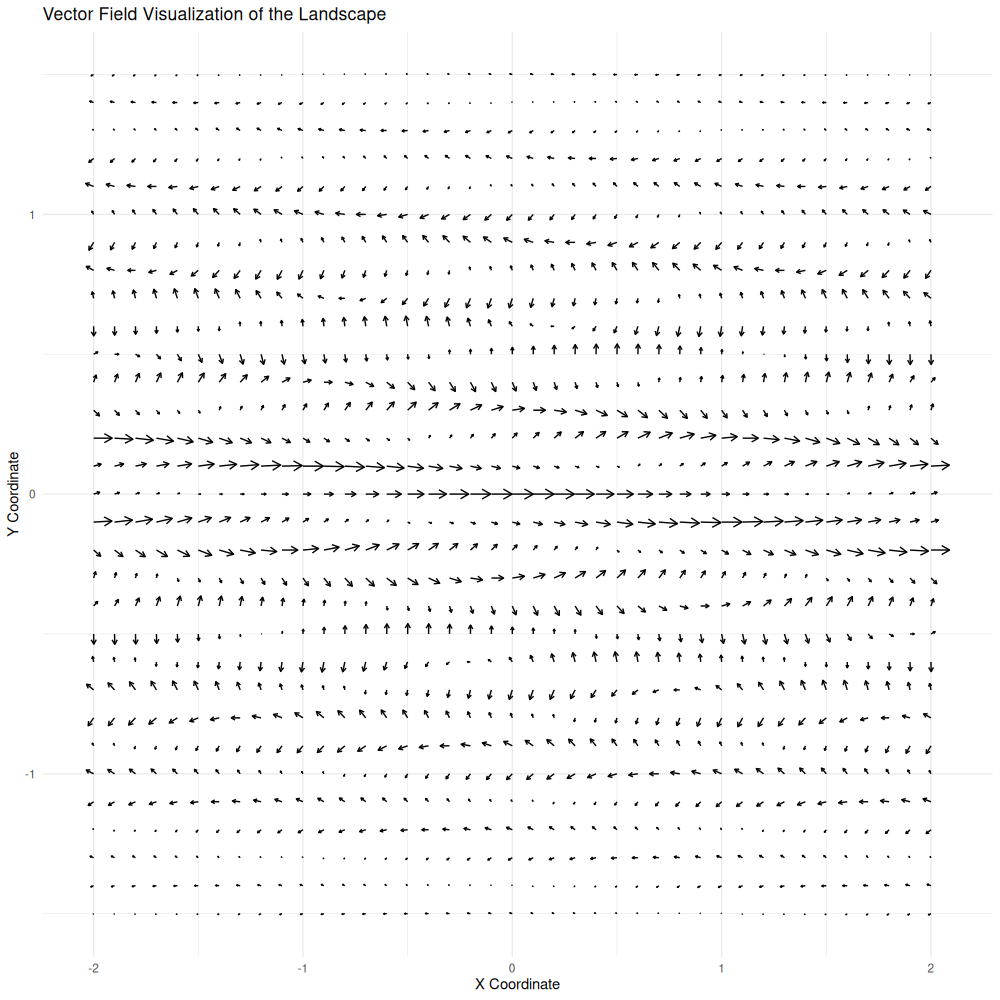
\includegraphics[width=\textwidth]{../Code/week 10/task1VectorField.png} 
\end{figure}



\subsection{Task 2}
Question: Integral vector field visualisation using streamlines (one good visualisation and one poor visualisation, as
described in Task 2).
\\
Answer: 

\begin{figure}[H]
\centering
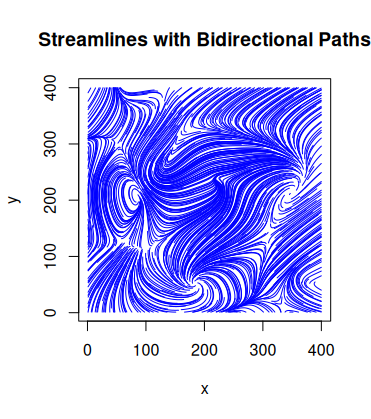
\includegraphics[width=\textwidth]{../Code/week 10/good streamline.png}
\caption{Good}
\end{figure}


\begin{figure}[H]
\centering
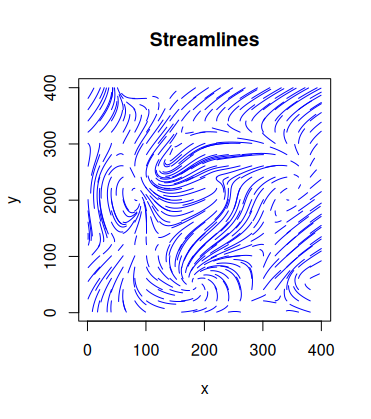
\includegraphics[width=\textwidth]{../Code/week 10/bad streamlines.png}
\caption{Bad}
\end{figure}



\subsection{Task 3}
Question: Line integral convolution for vector field visualisation (as described in Task 3).
\\
Answer: 
\begin{figure}[H]
\centering
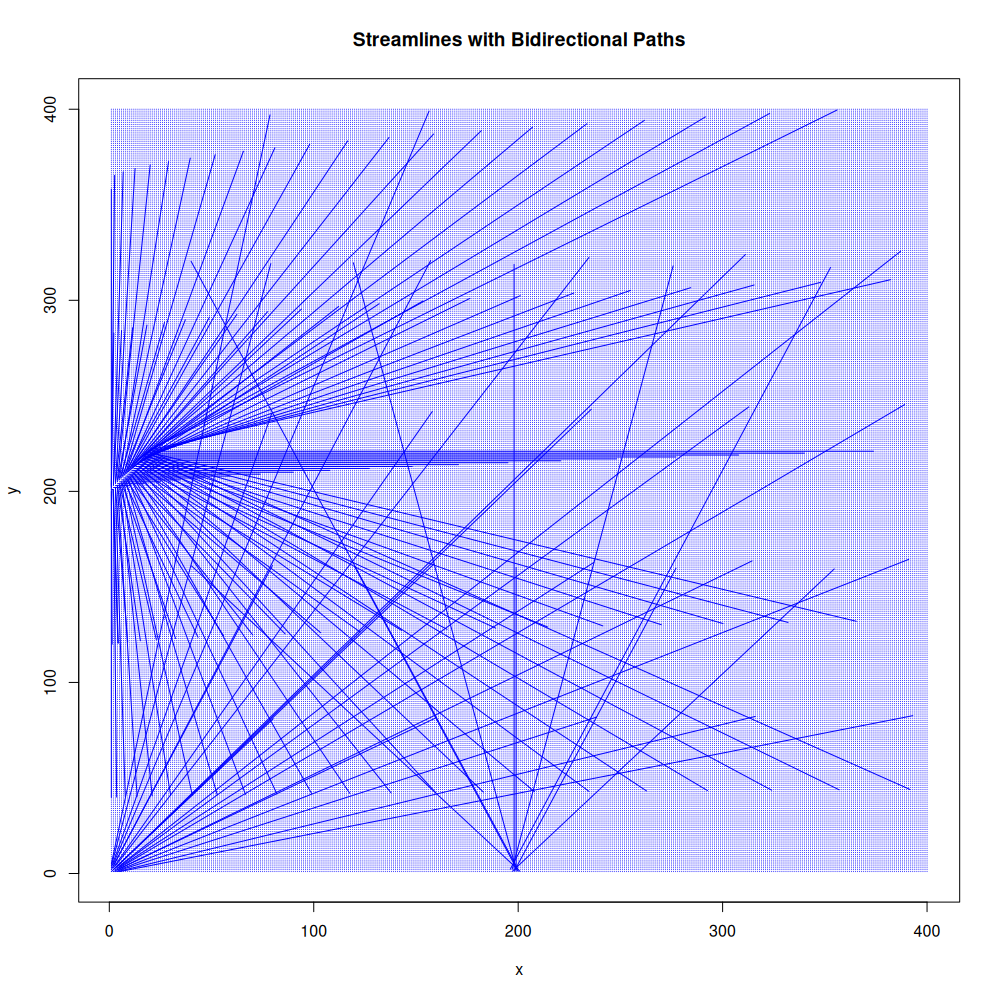
\includegraphics[width=\textwidth]{../Code/week 10/task3.png} 
\caption{Bad}
\end{figure}


\section{Week 12 - Visualising High Dimensional Data}
\subsection{Task 1}
Question: A scatter plot of each dimension of the dataset against each other dimension. Colour
code the different species.
\\
Answer: 

\begin{figure}[H]
\centering
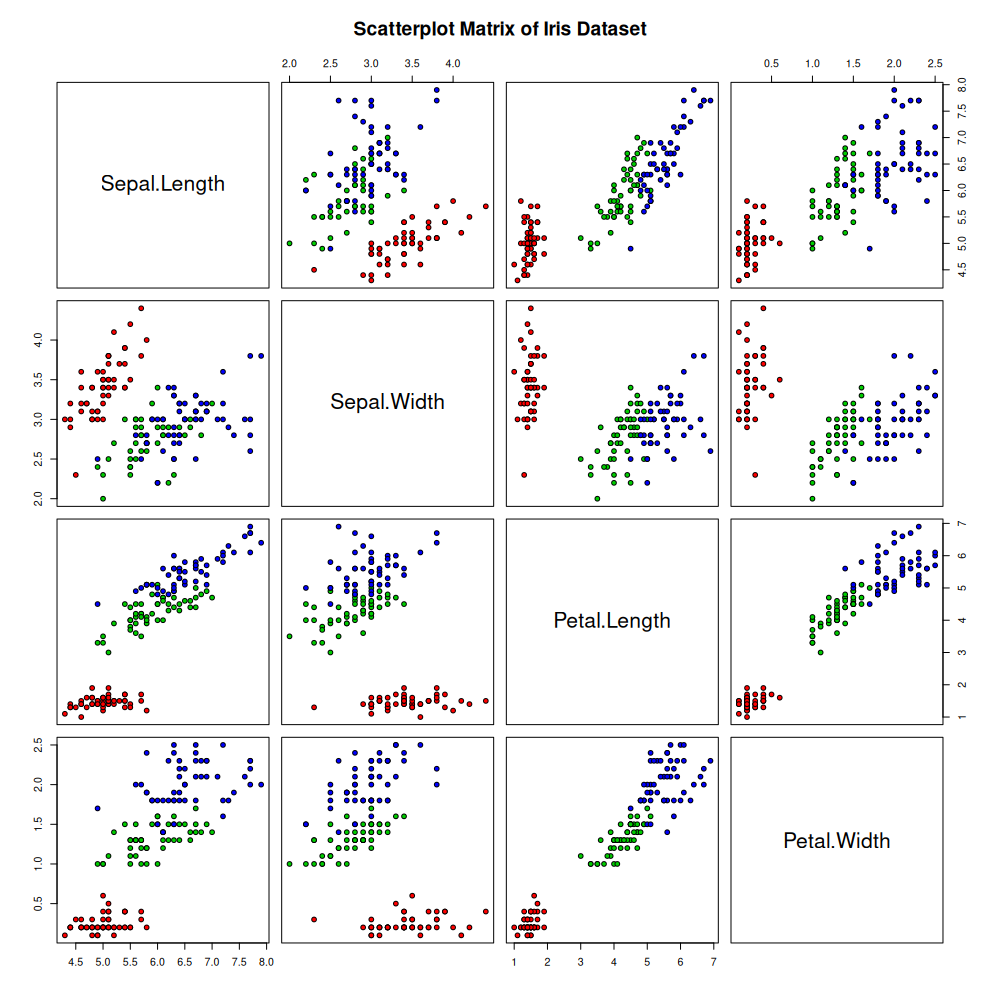
\includegraphics[width=\textwidth]{../Code/week12/task 1.png} 
\caption{Bad}
\end{figure}


\subsection{Task 2}
Question: A scatter plot of the data projected onto the two principal components that explain the
most variation.
\\
Answer: 

\begin{figure}[H]
\centering
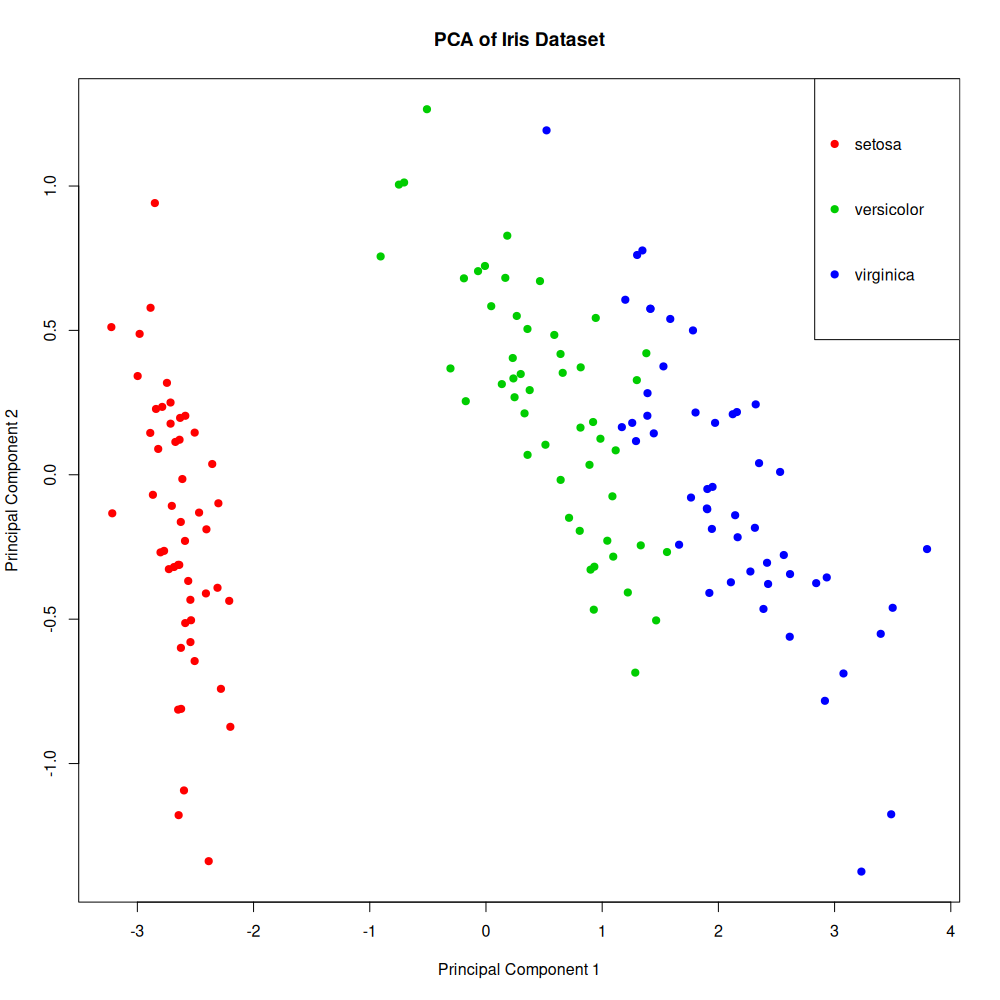
\includegraphics[width=\textwidth]{../Code/week12/task2.png}
\caption{Bad}
\end{figure}

\subsection{Task 3}
Question: Calculate a good projection vector for applying LDA to the first two dimensions of the
iris dataset. Report both the 2x1 vector W and the value of J(W).
\\
Answer: \\
Optimal Projection Vector W: 0.8267396 -0.5625848\\
Value of J(W): 4.171799 

\subsection{Task 4}
Question: A visualisation of the iris data along this projection vector, showing how it separates
the different species of flower.
\\
Answer:
\begin{figure}[H]
\centering
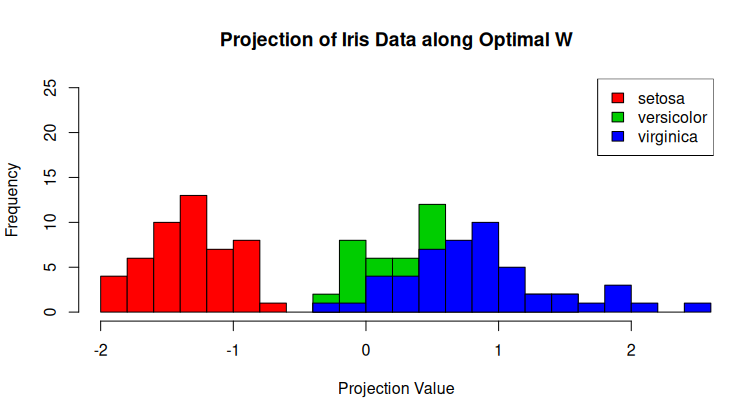
\includegraphics[width=\textwidth]{../Code/week12/task 3.png}
\caption{Bad}
\end{figure}


\end{document}